\chapter{Design}
\label{Design}
This chapter describes the proposed design of the whole system for storing and exploring blockchains in IPFS that is to be created as a result of this thesis. All parts of the system are described in this chapter.

\section{Database system}
We need a database in our system to store and index data. Database system needs to be decentralized and distributed. There are several databases build on top of IPFS already implemented. The two most known are OrbitDB and Textile.

\subsection{OrbitDB}
OrbitDB is a serverless, distributed, peer-to-peer database build on top of IPFS, developed by HAJA networks. OrbitDB is a decent solution for small user's databases, but it is still in the alpha stage of developing, and it is not well optimized to store hundreds of gigabytes of data. The biggest problem is that OrbitDB performs all queries locally. To perform a query that selects transactions that are more valuable than 1BTC, OrbitDB needs to load the whole database locally and then perform a cycle on all transactions to selects only those transactions that meet the criteria. So every client ends up with a full copy of the database. This limitation is not usable for our case when we have a database that has hundreds of gigabytes of data.

\subsection{Textile}
Textile is a set of open-source tools that provide a distributed peer-to-peer database, remote storage, user management, and more, over the IPFS network. Textile already created applications for storing photos, notes or anything else (Anytype). Textile provides a high abstraction on top of the IPFS and provides simple API to store and index files securely. It uses Cafe peers to provides backups and indexing. Data are duplicated on several Cafe peers. When a client is performing some query, it contacts one of the Cafe peers to resolve the query for the client.
Neither of these solutions fits our use case to store a large amount of data distributed on several nodes and performs queries that can be resolved by downloading only necessary parts of the database. Therefore, we need to create a new database system based on IFPS that would be decentralized and distributed.

\subsection{Database system design}
A database system that fits our needs is distributed and decentralized. That brings us lots of synchronization problems to solve. This database system consists of tables that contain records. For faster searching, tables have indexes. Relations between tables are represented via foreign keys. Also, this database system supports fluent query language, used for performing complex queries.

\subsubsection{Record} 
Every record in our database system is stored in an append-only log that contains the whole history of the record. Every update of a record adds a new entry to its log which points to the previous entry. 

In centralized systems such as git, conflicts are detected on write (for example, when two git users push changes to the server at the same time, one of them gets an error and needs to pull repository). This approach is impossible in a decentralized system. When we update some record in our database, we can not know if somebody does not update it before (and we do not receive changes yet). For this reason, we need to solve conflicts while reading. Record with conflict has more than one head on record log, and users need to solve them in application logic.


\subsubsection{Indexes}
An index is B-tree optimized for IPFS (no cycled references and node size less than 256kB). Each table has at least one primary index. Primary Index - We use the primary index to reference record in foreign keys. A primary key is automatically created when a user does not specify it. Value of the primary key for an entity can not be changed (because we would need to scan all tables where the entity is referenced and change the referenced value to a new one). Also, when we execute a query without any condition or sorting, we use a primary key to obtain records. Every index has several components: 
\begin{itemize}
    \item \textbf{Comparator} - is a function that has two parameters (two keys of B-tree) and outputs a number. An index is using a comparator to search records and insert record to the right place in B-tree.
    \item \textbf{Key-getter} - is a function that returns a comparable object from the record (a comparable object is an object that can be compared using index comparator). Every index has key-getter that is using to obtain keys for B-tree.
\end{itemize}

\subsubsection{Table}
A table contains indexes, a list of foreign keys and table name.

\subsubsection{Foreign keys}
We use foreign keys to represent relationships between tables. A foreign key is the value of a primary key of a referenced record.

\subsubsection{Transactions}
When we commit a transaction, it is inserted to the queue. If there are more transactions in the queue, a database performs it one by one.

\subsubsection{Synchronization} 
Every time a transaction queue is empty (all pending transactions has been applied), a new version of a database is broadcasted to all connected users. When we receive information about the new database version, we load its root. Each database version has information from which version was created. Database versions create an append-only log. 

If more than one user publishes a new version of the database that has been created from the same version, other use needs to decide which version they would accept. There are multiple ways to solve database version conflicts: 
\begin{itemize}
    \item Compare hashes of new database versions and who has the biggest hash wins,
    \item A user who is connected for the longest time wins.
\end{itemize}

\subsubsection{Queries} 
A Database system provides query language for performing selects. A query consists of:
\begin{itemize}
    \item \textbf{conditions} - query may contains multiple conditions. There are logical operators (and - conjunction, or - disjunction) between conditions. When it is possible (an index is available on condition property), we use indexes for evaluating conditions. If there are more than one conditions, we use an intersection between and's conditions and union between or's a disjunction. These types of conditions are supported:
    \begin{itemize}
        \item \textbf{equal} - record property equals to specified value,
        \item \textbf{greather than} - record property is greather than specified value,
        \item \textbf{less than} - record property is less than specified value,
        \item \textbf{between} - record property is greather than specified minimal value, and less than specified maximal value.
    \end{itemize} 
    \item \textbf{filters} - filters are similar to conditions, but they can be more complicated. They are functions returning boolean that are being applied to query results. If any filter return \texttt{false} for the query result, the query result is ignored. A query can contain several filters.
    \item \textbf{offset} - offset saying how many query results should be ignored from the beginning.
    \item \textbf{evaluator} - we use evaluator for accessing results of the query.
    \begin{itemize}
        \item \textbf{all} - all evaluator returns array of all results of the query,
        \item \textbf{first} - returns only first result,
        \item \textbf{take} - returns \texttt{N} number of results,
        \item \textbf{paginate} - 
        \item \textbf{iterate} -
    \end{itemize}
\end{itemize}  

\section{System components}
The system consists of one or more Feeders and Explorers. Feeders are connected to data sources and provide synchronization with cryptocurrency blockchains. Explorer can request data from the system network and display them to a user (see Figure \ref{systemArchitecture}).

\begin{figure}[h]
    \centering
    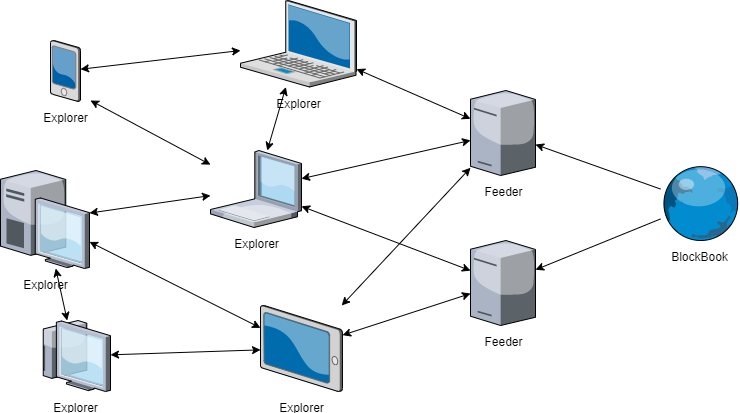
\includegraphics[width=11cm]{AppArchitecture.png}
    \caption{System design}
    \label{systemArchitecture}
\end{figure}

\section{Blockbook}
Blockbook\footnote{\url{https://github.com/trezor/blockbook}} is a blockchain indexer for Trezor Wallet\footnote{\url{https://wallet.trezor.io/}}, developed by SatoshiLabs\footnote{\url{https://satoshilabs.com/}}. It currently supports more than 30 coins (and the community implemented some others). For data storage Blockbook is using RocksDB\footnote{\url{https://github.com/facebook/rocksdb/wiki}} developed by Facebook, which is a NoSQL database which stores only key-value pairs. Blockbook is providing fast API for accessing blocks, addresses and transactions. Main limitations of blockbook:
\begin{itemize}
    \item \textbf{Not distributed} (client-server architecture) - problem with scaling for more users. 
    \item \textbf{Not a SQL database} - it does not have a relational data model, it does not support SQL queries, and it has no support for indexes.
    \item \textbf{Single-Process} - only a single process (possibly multi-threaded) can access a particular database at a time.
\end{itemize}

\section{Feeder}
A Feeder is a command-line service that stores data in IPFS for all cryptocurrencies specified in the config file. It uses Blockbook API for obtaining data. Feeder stores data in structure such as in Figure \ref{feederDataStorageStructure}. Each block (except genesis and last block) has a link to the previous and next block. Also, it has links to transactions that had been processed in this block. A transaction has links to address and previous/spent transaction for every input/output. This scheme allows to store blockchain data in IPFS in small objects with size less than 256kB (a limit for storing objects directly in DHT). Also, every logical link between objects is preserved.

\begin{figure}[h]
    \centering
    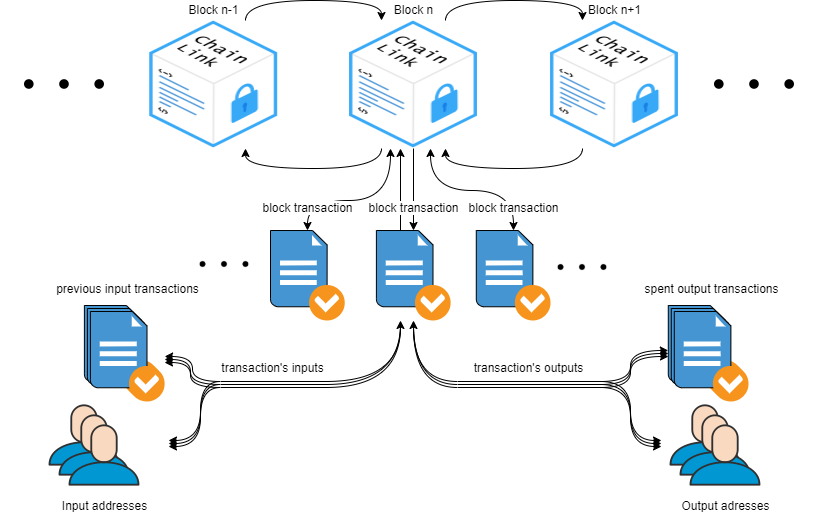
\includegraphics[width=12cm]{feederDataStorageStructure.png}
    \caption{Feeder data storage structure}
    \label{feederDataStorageStructure}
\end{figure}



\section{Explorer}
Explorer can perform basic queries like a search for block by its height or hash and search address and transaction by hash. Nevertheless, Explorer can also make more complex queries, for example, get 20 transaction where the sum of inputs is more than 0.5, or get transactions between some time interval. Explorer is an application that can be used in two environments. In browser with simple GUI, or in node.js\footnote{\url{https://nodejs.org/}} as a RestAPI.

\subsection{ExplorerGUI}
ExplorerGUI is browser version of Explorer. It is implemented as a SPA\footnote{\url{https://en.wikipedia.org/wiki/Single-page_application}} to prevent restarting connection with IPFS. It has separated views for block, transaction and address details. Also paginating, filtering and sorting objects by all its properties is supported.

\subsection{ExplorerAPI}
\label{explorerAPIroutes}
ExplorerAPI is a node.js application provides several endpoints for obtaining the data:
\begin{itemize}
    \item \texttt{GET /tx} - get collection of transaction, 
    \item \texttt{GET /tx/[:txHash]} - get transaction by hash,
    \item \texttt{GET /block} - get block collection,
    \item \texttt{GET /block/[:blockHeightOrHash]} - get block by height or hash,
    \item \texttt{GET /address} - get address collection,
    \item \texttt{GET /address/[:hash]} - get address by hash.
\end{itemize}
All endpoints support more detailed path specification by providing multiple parameters at the end of the path (for example, it is possible to request only a block hash by calling \texttt{/block/42/hash}). Also, every endpoint supports query parameters
\begin{itemize}
    \item \texttt{filter} where value of this parameter can be simple arithmetic expression like \texttt{height>50},
    \item \texttt{limit} parameter for pagination with default value set to \texttt{20},
    \item \texttt{orderBy} sorts results of a sequence in ascending order.
\end{itemize}
 



